\section{Results} \label{sec:cba_results}
With the aircraft maneuver and flight simulation process defined, results from running the GTT aircraft through the flight certification maneuver are discussed in this section.
There are two over-arching goals of this work: first, to provide a framework that brings flight testing earlier in the aircraft design process, and second, to create the most accurate flight simulation results while minimizing the cost of the underlying analyses. 
To this end, this section first focuses on comparing simulations that are run using purely high-fidelity experimental data, to those run using low-fidelity and multi-fidelity data that would be available early in the design process.
Then the cost-reduction aspect is explored by harnessing the benefits of multi-fidelity databases that use small subsets of the high-fidelity data. 
For all the results in this section, simulations are conducted with the right engine inoperative, and all modifications discussed in Section \ref{subsec:sim_mods} are applied.

\subsection{Simulations using Single- vs. Multi-Fidelity Databases} \label{subsec:sf_vs_mf_cba}

In the nascent stages of the aircraft design, low-fidelity methods, such as AVL simulations, are used to perform rapid analyses that can span wide regions of the design domain quickly. 
These have higher uncertainties in their performance predictions due to simplifications made in modeling the flow physics, in favor of speed of analysis.
As parts of the aircraft design are fixed, higher-fidelity methods such as RANS CFD simulations are used to perform design optimizations.
These are computationally more expensive than AVL simulations, but also provide a more accurate representation of the aircraft's potential performance. 
Once designs are finalized, prototypes that can be experimentally tested in wind tunnels, are manufactured. 
These provide high-fidelity data that can recreate the expected flight conditions and have correspondingly low uncertainties associated with their performance predictions.
Finally, flight testing to certify the aircraft's air-worthiness is performed once all the design decisions are finalized and a full-sized prototype is manufactured.

Mimicking this sequence of design analyses, single- and multi-fidelity databases that use, in order, low-fidelity (AVL), low- + medium-fidelity (AVL + SU2), and low- + medium- + high-fidelity (AVL + SU2 + WT) data are created. 
An example of this build-up is presented in Section \ref{sec:data_gen}.
To bring aspects of the real-world flight testing procedure into the virtual environment where early design analyses are performed, flight simulations are carried out using these lower fidelity databases.
To assess the quality of the results, these are compared to flight simulations carried out using high-fidelity databases created using only the available wind tunnel data. 
It is important to note that while wind tunnel data has its own set of models that introduce errors when compared to flight tests, it is the highest-fidelity data available and is considered the truth function that is being emulated. 

It is important to remember that only basic aerodynamic coefficient data is available from SU2. 
This means that the two-fidelity results only use SU2 data for the force and moment coefficients in the aerodynamics database.
The controls databases for the two-fidelity results are actually only single-fidelity and are identical to the controls databases used for the AVL-only results. 
Consequently, the three-fidelity database is only truly three-fidelity for the force and moment coefficients; the rest are two-fidelity.
To avoid verbose explanations, the overall results are still referred to as two-fidelity when AVL+SU2 data is used, and three-fidelity when AVL+SU2+WT data is used. 

\begin{figure}
    \centering
    \begin{subfigure}[CDF for the trim $\alpha$]{
        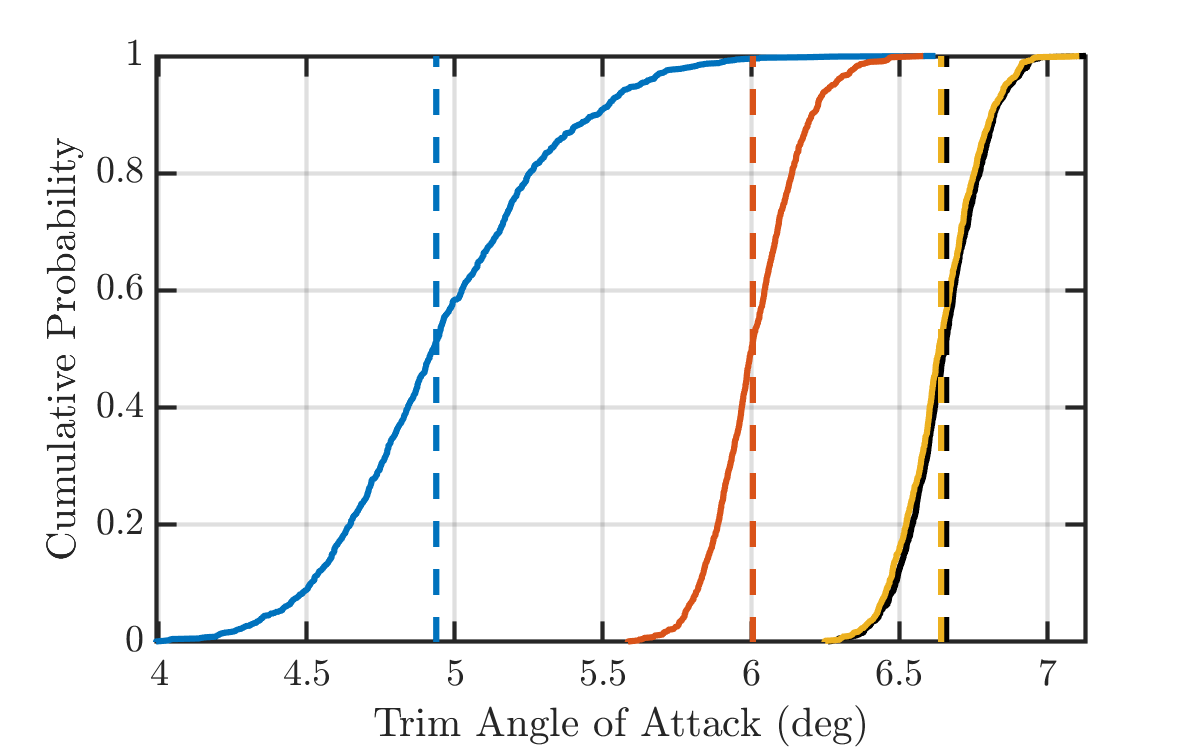
\includegraphics[trim=0 0 0 0, clip, width=.48\textwidth]{code/image_gen/cba/Stanford_CFR25_147d_2_R2/images/trim_aoa_sf_vs_mf.png} 
        \label{subfig:sf_vs_mf_trim_cdf}
    } 
    \end{subfigure}
    \hfill
    \begin{subfigure}[CDF for the pitch metric]{
        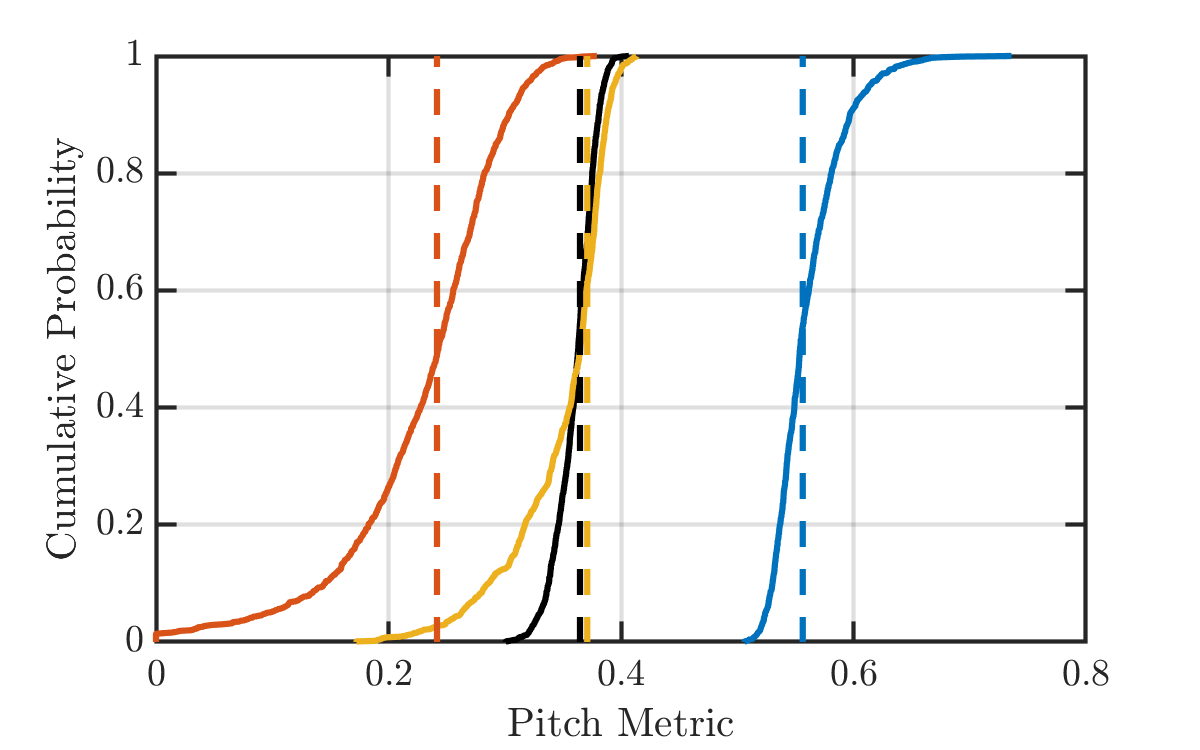
\includegraphics[trim=0 0 0 0, clip, width=.48\textwidth]{code/image_gen/cba/Stanford_CFR25_147d_2_R2/images/reo_pitch_sf_vs_mf.png} 
        \label{subfig:sf_vs_mf_pitch_cdf}
    } 
    \end{subfigure}
    \hfill
    \begin{subfigure}[CDF for the roll metric]{
        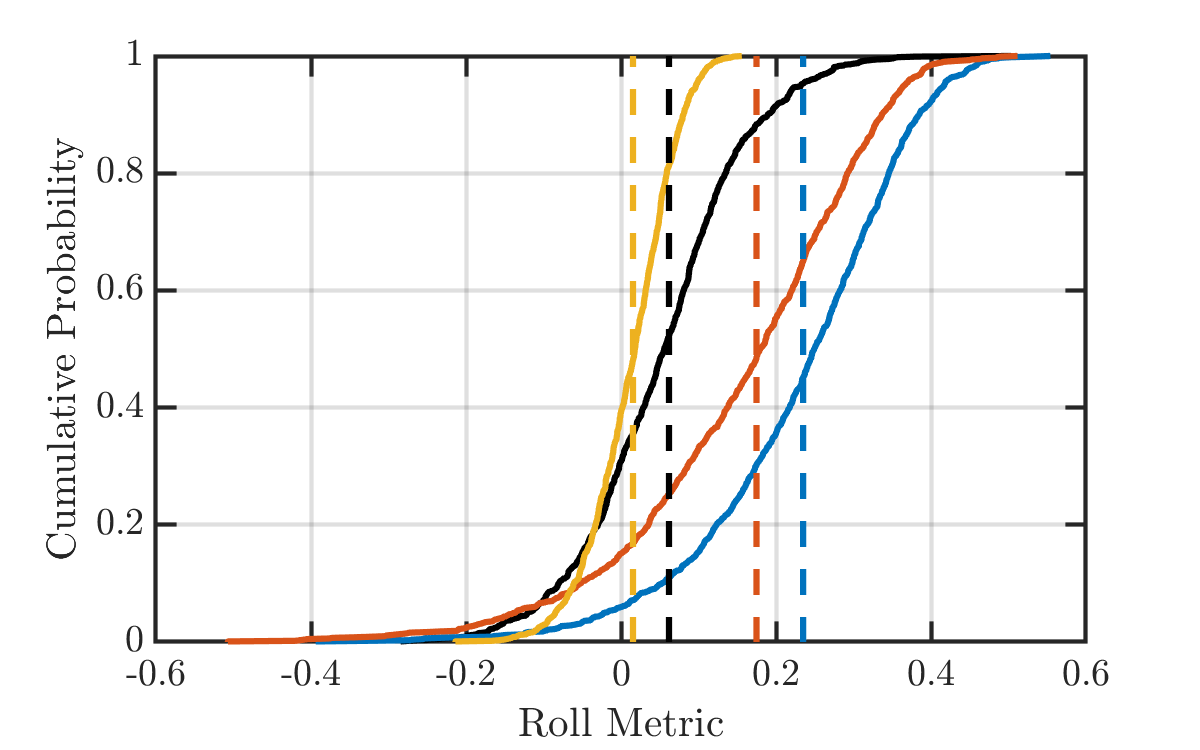
\includegraphics[trim=0 0 0 0, clip, width=.48\textwidth]{code/image_gen/cba/Stanford_CFR25_147d_2_R2/images/reo_roll_sf_vs_mf.png} 
        \label{subfig:sf_vs_mf_roll_cdf}
    } 
    \end{subfigure}
    \hfill
    \begin{subfigure}[CDF for the yaw metric]{
        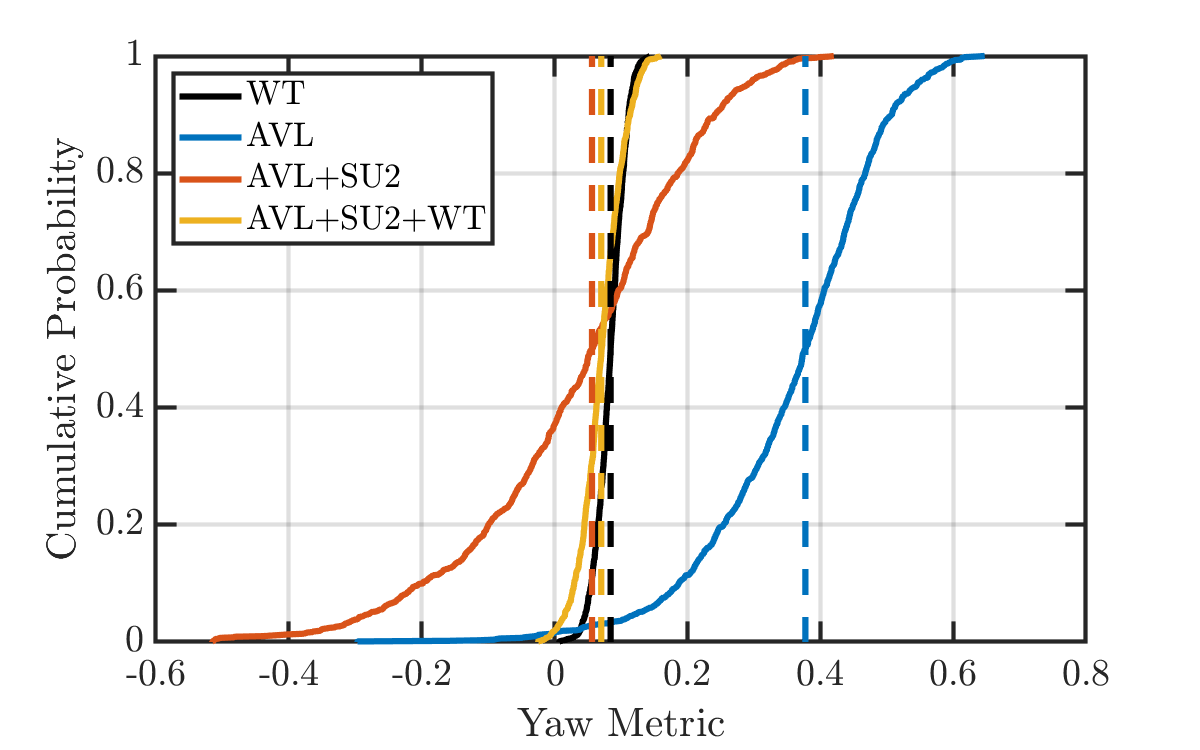
\includegraphics[trim=0 0 0 0, clip, width=.48\textwidth]{code/image_gen/cba/Stanford_CFR25_147d_2_R2/images/reo_yaw_sf_vs_mf.png} 
        \label{subfig:sf_vs_mf_yaw_cdf}
    } 
    \end{subfigure}
    \caption{Comparing flight simulations of the certification maneuver when different combinations of low-, multi-, and high-fidelity databases are used. CDF plots for the trim angle of attack and the success metrics are shown. \label{fig:sf_vs_mf_metric_cdfs}}
\end{figure}

With the details of the simulation procedure explained in Section \ref{sec:sim_procedure}, the results here will be presented primarily through the CDF plots of the success metrics resulting from the Monte Carlo analysis defined in \ref{subsec:mc_analysis}.

Figure \ref{fig:sf_vs_mf_metric_cdfs} presents the results of the flight simulations when lower fidelity databases are used.
Early in the conceptual design stages, the aircraft performance would be determined using low-fidelity analyses and the flight simulations would yield the results represented by the blue line. 
The large uncertainties attributed to the AVL analyses yields large variance in the metrics, indicated by the wide range of values that the CDF spans for every metric. 
AVL also over-predicts the effectiveness of all control surfaces.
The CDF for each metric lies to the right of the other results, indicating lower control surface saturation during the course of the simulations. 

Progressing with the aircraft design, when RANS CFD data is added to the GP models, the results of flight simulations are represented by the red line. 
The effect of having more accurate aerodynamic force and moment coefficients is evident, especially in calculating the trim angle of attack shown in Figure \ref{subfig:sf_vs_mf_trim_cdf}.
Since no additional data is used to improve the controls databases, the large variance in success metrics is seen with these two-fidelity results as well. 
Nevertheless, the additional accuracy in the baseline aerodynamics shifts all of the two-fidelity results closer towards the three-fidelity and high-fidelity results.

With the addition of the wind tunnel data to the multi-fidelity fit (yellow line), the flight simulation results should be very close, if not identical, to those using the single-, high-fidelity data (black line). 
The trim angles of attack, pitch metrics, and yaw metrics line up identically, there is a notable difference in the roll metric results. 
Not only is the mean value for the three-fidelity database (dashed yellow line) lower than that for the single-, high-fidelity database, but the variance in the roll metric is also lower. 
The reason for this difference was hinted at in Section \ref{sec:gtt_dbs} when comparing the single- and multi-fidelity databases for $C_{l{\delta_a}}$. 
This is highlighted in Figure \ref{fig:sf_vs_mf_crmail} when plotting samples of the databases as a function of $\delta_a$ when $\alpha=8^\circ$ and $\beta = 4^\circ$.

\begin{figure}
    \centering
    \begin{subfigure}[Single-, high-fidelity database]{
        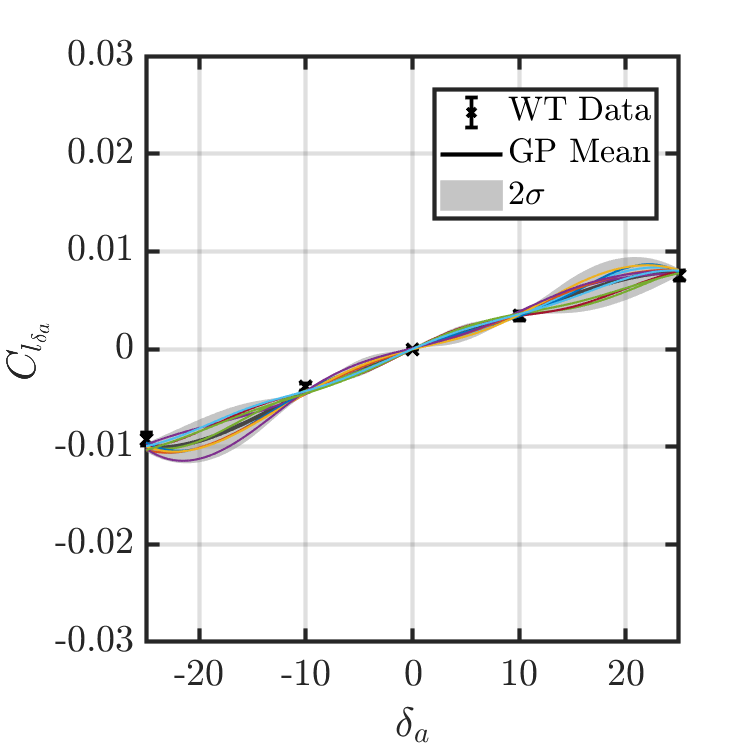
\includegraphics[trim=0 0 0 0, clip, width=.48\textwidth]{code/image_gen/gmatt/1f/wt_old/images/gps/CRMAIL_alpha=8_beta=4+samps.png} 
        \label{subfig:sf_crmail}
    } 
    \end{subfigure}
    \hfill
    \begin{subfigure}[Multi-fidelity database]{
        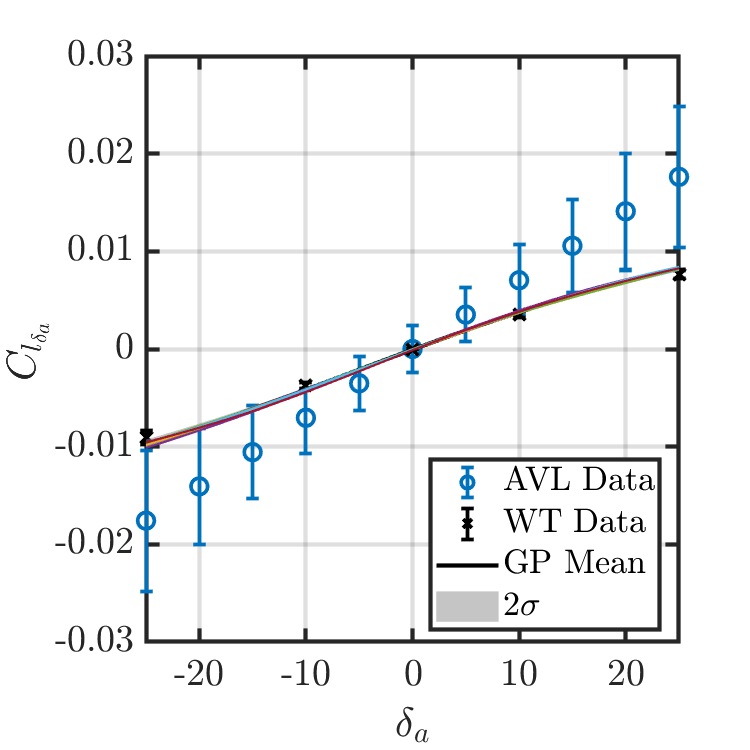
\includegraphics[trim=0 0 0 0, clip, width=.48\textwidth]{code/image_gen/gmatt/3f/images/gps/CRMAIL_alpha=8_beta=4+samps.png} 
        \label{subfig:mf_crmail}
    } 
    \end{subfigure}
    \caption{Comparing $C_{l{\delta_a}}$ as a function of $\delta_a$ when single-, high-fidelity data is used vs. when multi-fidelity data is used. The individual colored lines represent samples of the database. \label{fig:sf_vs_mf_crmail}}
\end{figure}

When only wind tunnel data is used to create the database, Figure \ref{subfig:sf_crmail}, the sparsity of data points in the aileron deflection dimension results in the ballooning GP error estimate between available data points (the black squares).
The database samples, $10$ of which are shown by the individual colored lines,  respect the error estimate from the GP and have correspondingly higher variability between those data points.
If the wind tunnel data is supplemented with lower-fidelity AVL data (blue circles), the multi-fidelity GP is able to use the trends learned from the lower fidelity to reduce the uncertainty between the same wind tunnel data points. 
As a result, the error estimate from the GP is much lower and can barely be discerned at the scale of the figure. 
The samples show significantly less variation from the mean database and are almost all coincident in this case. 
This reduction in sample variation corresponds to the lower variation indicated by the CDF plot for the three-fidelity roll metric in Figure \ref{subfig:sf_vs_mf_roll_cdf}.





The black line represents the results using the high-fidelity GP models that only use wind tunnel data. 
Across all the metrics, adding levels of fidelity bring the results closer to the sing
